Die gewohnte Bewegungsfreiheit in der erweiterten Realität beizubehalten ist bei weitem nicht trivial.
Zwar ist der Körper nicht eingeschränkt und es kann problemlos durch die durchsichtigen Gläser von AR-Headsets gesehen werde, allerdings bewegt sich der Ursprung des bekannten Koordinatensystems.

Die schwierigkeit liegt also darin, Objekte im realen Raum platzieren zu können.
\footnote{Ein weiteres großes problem, mit dem wir uns an dieser Stelle nicht befassen wollen, ist die Interaktion mit diesen objekten, also das Body Tracking.}

\subsection{Degrees Of Freedom}\label{subsec:degrees-of-freedom}
    Degrees Of Freedom~\autocite{wikipedia-contributors-2023B}, kurz \textbf{DOF}, bezeichnen die Bewegungsfreiheiten eines Systems in einem Vektorraum.
    Ein einfaches Beispiel sei mit der klassischen Transformationsmatrix in \autoref{fig:matrix-DOFs} gegeben.
    \begin{figure}[ht!]
        \label{fig:matrix-DOFs}
        \begin{center}
            \begin{math}
                \begin{bmatrix}
                {\color{red} s}
                    \cdot {\color{green} t_{1,1}} & {\color{green} t_{1,2}}                       & {\color{green} t_{1,3}}                       & {\color{blue} v_x} \\
                    {\color{green} t_{2,1}}       & {\color{red} s} \cdot {\color{green} t_{2,2}} & {\color{green} t_{2,3}}                       & {\color{blue} v_y} \\
                    {\color{green} t_{3,1}}       & {\color{green} t_{3,2}}                       & {\color{red} s} \cdot {\color{green} t_{3,3}} & {\color{blue} v_z} \\
                    0                             & 0                                             & 0                                             & {\color{red} s}
                \end{bmatrix}
            \end{math}
        \end{center}
        \begin{tabular}{c|c|c}
            var             & Bezeichnung & DOF \\
            \hline
            \color{red} s   & Skalar      & 1   \\
            \color{blue} v  & Vektor      & 3   \\
            \color{green} t & Tensor      & 6   \\
        \end{tabular}
        \caption{Degrees Of Freedom der Transformationsmatrix}
    \end{figure}
    Ein DOF bezeichnet dabei einen eindimensionalen Parameter des Systems.
    Es wird also mit jedem Parameter ein größerer Vektorraum aufgespannt.
    Der DOF entspricht damit der Dimension des zugehörigen Vektorraumes.

    Der visuell einfachste Teilraum aus \autoref{fig:matrix-DOFs} ist das kartesische Koordinatensystem, hier bezeichnet als \textbf{Vektor}.
    Im dreidimensionalen Raum ist eine Bewegung in 3 Richtungen möglich.

    Dazu kommt die \textbf{Skalierung}.
    Auch diese sollte leicht verständlich sein.

    Komplizierter wird die \textbf{Tensor}-Transformation.
    Diese bezeichnet die Kombination aus \textbf{Rotation} und \textbf{Scherung}.
    Diese sind jeweils um alle 3 Achsen des kartesischen Koordinatensystems möglich und haben damit jeweils 3DOF\@.
    Daraus ergeben sich 10DOF der klassischen Transformationsmatrix.

    AR-Headsets sin allerdings deutlich eingeschränkter.
    Sie haben 6DOF~\autocite{wikipedia-contributors-2023B}.

    Das physische headset kann sich, wie in \autoref{fig:6DOF} dargestellt, im Raum von $\vec{a}$ nach $\vec{b}$ bewegen und um jede seiner Achsen rotieren, allerdings nicht geschert oder skaliert werden.
    \begin{figure}[ht!]
        \label{fig:6DOF}
        \center
        \includesvg[width={0.5\textwidth}]{../assets/img/6DOF}
        \caption{6 Degrees Of Freedom~\autocite{wikipedia-contributors-2023B}}
    \end{figure}
    Damit wird die Darstellung meistens auf einen Vektor für die Position sowie eine Quaternion~\autocite{wikipedia-contributors-2023G} für die Rotation beschränkt.

\subsection{Positioning System}\label{subsec:positioning-system}
    Das bringt die Entwicklung von AR-Headsets vor seine ganz eigene Herausforderung, da diese 6DOF notwendig sind, um dem nutzer ein minimum an Orientierung zu bieten.

    Dazu werden Positionierungssysteme~\autocite{wikipedia-contributors-2023A} verwendet.

    \subsubsection{Global Positioning System}\label{subsubsec:global-positioning-system}
        Eines der bekanntesten Positionierungssysteme ist das GPS~\autocite{wikipedia-contributors-2023J}, welches heutzutage in jedem Mobiltelefon verbaut ist.
        GPS ist eines der wenigen globalen Satellitennavigationssysteme.

        Diese Systeme lösen das Problem der Positionierung, wie der Name suggeriert, indem, mindestens 4, Satellite, in Sichtweite, Radiowellen wellen aussenden.
        Die Radiowellen tragen als Signal den Zeitstempel des senden des Signals, damit ist der Abstand vom Empfänger zum Sender von allen Satellite in Sichtweite bekannt.
        \begin{figure}[ht!]
            \label{fig:ToF}
            \center
            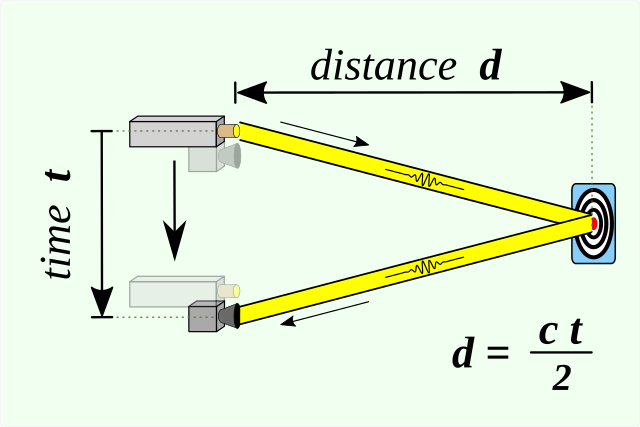
\includegraphics[width={0.5\textwidth}]{../assets/img/time_of_flight}
            \caption{Time of Flight~\autocite{wikipedia-contributors-2023D}}
        \end{figure}
        Dieses Konzept wird Time of Flight~\autocite{wikipedia-contributors-2023D}, kurz \textbf{ToF}, genannt und ist in \autoref{fig:ToF} dargestellt.

        Dem aufmerksamen Leser sollte aufgefallen sein, dass 4 weniger als 6 ist.
        Deshalb können aus den 4 Zahlen auch nur 3DOF, also die Position, auf 0.3 bis zu 5 Meter genau, errechnet werden.

    \subsubsection{Indoor Positioning System}\label{subsubsec:indoor-positioning-system}
        Aufgrund dieser Ungenauigkeit kann GPS auch nicht für die ersten 3DOF genutzt werden.
        Auch mit 30~cm ungenauigkeit könnten wir in keine virtuelle Realität eintauchen.

        Deshalb müssen genauere Systeme her, sogenannte Indoor Positioning Systems~\autocite{wikipedia-contributors-2023E}.
        Diese sind Systeme, die die Positionierung innerhalb eines Raums oder Arbeitsplatzes ermöglichen.
        Ob 6DOF oder lediglich 3DOF erreicht werden ist dabei vom jeweiligen System abhängig.

        \paragraph{Base Stations}\label{par:base-stations} werden hierfür klassischerweise verwendet.
            Diese sind externe Geräte, welche, ähnlich wie die Satellite beim GPS, die Position des Empfängers ermitteln.

            Es gibt einige enterprise Systeme, welche zum Beispiel in Lagerhäusern verwendet werden~\autocite{wikipedia-contributors-2023E}.
            Für diese Ausarbeitung werden wir uns allerdings als Beispiel die SteamVR Base Station 2.0~\autocite{valve-corporation-no-date} anschauen.

            Diese nutzen allerdings keine Time of Flight.
            Anstatt die Position aus der Distanz zu errechnen wird hier die Position durch das Abtasten mittels eines Lasers ermittelt.
            Damit werden mehrere markante Punkte an dem VR-Headset pro Basisstation abgetastet.
            Es ergeben sich daraus also 6DOF\@.

        \paragraph{Spatial cognition}~\autocite{wikipedia-contributors-2023F} ist die Warnehrung der Umgebung vom Menschen und anderen Lebewesen.
            Unter anderem umfasst dieses Thema die Objektpermanenz.

            Als ein bionischer Ansatz wird dieses Konzept heute auf AR-Headsets angewendet.
            Daraus ergeben sich 6DOF, ohne an einen zuvor eingerichteten Raum gebunden zu sein.
            Die funktionalität solcher Systeme ist in \autoref{subsec:spatial-cognition-fuer-ar-headsets} beschrieben.

\subsection{Spatial Cognition beim Menschen}\label{subsec:spatial-cognition-beim-menschen}
    Das Kernkonzept der Spatial Cognition ist das Verarbeiten von Wissen über die Umgebung. \autocite{wikipedia-contributors-2023F}
    Es wird dabei regelmäßig neu organisiert, um das Verständnis der Umwelt zu verbessern.

    Als ein Beispiel wollen wir uns anschauen, wie Menschen ihre Umgebung beschreiben.
    Die wahrnehmung der Umgebung, spezieller ihre Darstellung, wie in \autoref{subsubsec:cognitive-map} weiter beschrieben, wird weitestgehend von der Sprache beeinflusst. \autocite{haviland-1998}
    Ich, so wie die meisten Leser vermutlich auch, sehe vor mir meinen Laptop, an dem ich dieses Paper schreibe.
    Für einen Sprecher der indigenen Sprache Guugu Yimithirr wäre mein Laptop südöstlich von mir.
    Das heißt, für uns ist die eigene orientierung im Raum wichtiger für die eigene Wahrnehmung.

    Um kurz in die Computergrafik zurückzukehren, ein Vergleich wäre das World Coordinate System für uns und das Camera Coordinate System für Guugu Yimithirr sprecher.

    Wir versetzen uns gerne in andere hinein, das ist aber ungünstig für Jagen oder Kämpfen in einer Formation.
    Während die Spatial Cognition bei Lebewesen zahlreiche Fachbereiche der Biologie und Psychologie abdeckt, stellt sich für uns die Frage, welche Informationen für den Nutzer am wichtigsten sind, um nicht die Orientierung zu verlieren, sowie welche Darstellungsformen wir übernehmen können, um die klassische Transformationsmatrix dieses Systems zu befähigen.

    \subsubsection{Navigation}\label{subsubsec:navigation}
        Diese beiden Systeme nennt man \enquote{Egocentric Navigation}\footnote{Beschreiben aus der Ich--Perspektive} und \enquote{Allocentric Navigation}\footnote{Beschreiben von einem allgemeinen Referenzpunkt}. \autocite{wikipedia-contributors-2023F}

        Zum Navigieren in großen, unbekannten Umgebungen ist dabei die Allocentric Navigation von Vorteil.
        Es werden große Referenzpunkte in der Landschaft gesucht und anhand eines globalen Koordinatensystems (Kompass) Richtungen angegeben.
        Die Abdeckung der Navigation ist damit höher.

        In bekannten Umgebungen ist die Egocentric Navigation allerdings im Vorteil.
        Vor allem lokale Objekte und der navigierende selbst werden als Referenz verwendet zusammen mit relationalen Begriffen wie \enquote{Links} oder \enquote{Rechts}.
        Da sich nicht so viele Sachen gemerkt werden müssen ist diese Art der Navigation effizienter, auf kosten der Effektivität.

    \subsubsection{Proprioception}\label{subsubsec:proprioception}
        Proprioception ist die Wahrnehmung des eigenen Körpers. \autocite{wikipedia-contributors-2023H}
        Spezifischer: die Wahrnehmung der eigenen Muskeln.

        Dadurch, dass die Ausdehnung jedes Muskels im Körper bekannt ist, wissen wir auch mit geschlossenen Augen, wo unser z.B.\ unser Arm ist.

        Diese Informationen fließen über das zentrale Nervensystem entweder in das Bewusstsein oder das Unterbewusstsein.
        Hier wird aus diesen Informationen, zusammen mit den anderen Sinnen, wie z.B.\ Sehen, Hören, Riechen oder der Gleichgewichtssinn; eine \enquote{Karte} von unserer Umgebung und unserer Körperposition erstellt.

    \subsubsection{Cognitive Map}\label{subsubsec:cognitive-map}
        Diese Cognitive Maps~\autocite{wikipedia-contributors-2023I} nutzen das sogenannte \enquote{Spatial Knowledge}, also all die zuvor beschriebenen Informationen, und bilden daraus eine abstrakte Darstellung.
        Diese wird umgangssprachlich manchmal als inneres Auge bezeichnet.

        \enquote{Map} ist hierbei nicht als Karte zu verstehen, sondern als Abbildung.
        Auch wenn es das anschaulichste Beispiel ist, weshalb wir uns in dieser Arbeit darauf begrenzen, können jegliche informationen auf diese Art und Weise abstrakt dargestellt werden.

        Handelt es sich um eine karten--ähnliche Struktur, so setzt sie sich, unter anderem, aus zwei Arten von Information zusammen:
        \begin{enumerate}
            \item Positional Landmarks\\
            Landmarks, oder Referenzpunkte, geben einen Uhrsprung für Wissen über die Umgebung.
            \item Directional Cues\\
            Richtungsangaben spezifizieren Relationen zwischen Objekten.
        \end{enumerate}

    \subsubsection{Reference Frames}\label{subsubsec:reference-frames}
        In \autoref{subsubsec:navigation} haben wir die Begriffe \enquote{Egocentric Navigation} und \enquote{Allocentric Navigation} kennen gelernt.
        Jetzt wollen wir diese Begriffe etwas verallgemeinern, damit wir sie später auch mittels Software formalisieren können.

        Um sich im Raum zurechtzufinden, also Spatial Knowledge zu besitzen, muss es immer einen Referenzpunkt \autocite{wikipedia-contributors-2023F}, genauer ein Referenzkoordinatensystem geben.
        Wir wissen bereits, dass diese Referenz die Ich--Perspektive\footnote{Beim Menschen ist es die Egocentric Navigation, in der VR sind es HUDs}, signifikante Punkte in der Landschaft\footnote{Beim Menschen ist es die Allocentric Navigation, in der VR sind es Base Stations} oder das Magnetfeld der Erde\footnote{Beim Menschen ist es der Kompass, in der Technik GPS} sein können.
        Dies sind aber nicht die einzigen Optionen.

        Ein nennenswertes Problem ist die Navigation im Weltraum.
        Hier wird meistens ein Gitter mit einem frei gewählten Nullpunkt verwendet.

        Allerdings ist das Referenzsystem beim Menschen dynamisch und individuell.
        Auch wenn nur wenige formularisiert sind, so gibt es sehr viele mehr.

\subsection{Spatial Cognition für AR-Headsets}\label{subsec:spatial-cognition-fuer-ar-headsets}

    \subsubsection{World Coordinate System}\label{subsubsec:world-coordinate-system}

    \subsubsection{Spatial anchors}\label{subsubsec:spatial-anchors}

    \subsubsection{Stationary frame of reference}\label{subsubsec:stationary-frame-of-reference}

        \paragraph{Knowledge engineering}~\autocite{wikipedia-contributors-2023C}